\documentclass[sigconf]{acmart}

\usepackage[english]{babel}
\usepackage{blindtext}

% Copyright
\renewcommand\footnotetextcopyrightpermission[1]{} % removes footnote with conference info
\setcopyright{none}
%\setcopyright{acmcopyright}
%\setcopyright{acmlicensed}
%\setcopyright{rightsretained}
%\setcopyright{usgov}
%\setcopyright{usgovmixed}
%\setcopyright{cagov}
%\setcopyright{cagovmixed}

\settopmatter{printacmref=false, printccs=false, printfolios=true}

% DOI
\acmDOI{}

% ISBN
\acmISBN{}

%Conference
%\acmConference[Submitted for review to SIGCOMM]{}
%\acmYear{2018}
%\copyrightyear{}

%% {} with no args suppresses printing of the price
\acmPrice{}


\begin{document}
\title{ATR: Additional Truncated Packets for Large DNS Response }

%\titlenote{Produces the permission block, and copyright information}
%\subtitle{Extended Abstract}

\author{Linjian Song, Shengling Wang}
% \author{Firstname Lastname}
% \authornote{Note}
% \orcid{1234-5678-9012}
% \affiliation{%
%   \institution{Affiliation}
%   \streetaddress{Address}
%   \city{City} 
%   \state{State} 
%   \postcode{Zipcode}
% }
% \email{email@domain.com}

% The default list of authors is too long for headers}
\renewcommand{\shortauthors}{X.et al.}

\begin{abstract}
   Internet works on reliable naming and IP package transmission. 
   As complexity added into Internet infrastructure due to security 
   and stability consideration, some mismatch and unexpected fragility 
   are exposed. One case is in the field of DNS (DNSSEC) and IPv6. 
   There are some public evidence and concerns on IPv6 fragmentation 
   issues due to larger DNS payloads over IPv6. Different from other 
   measurement work, in this paper we proposed "glueless" measurement 
   mechanism to analyze the end-to-end users experience worldwide. 
   It is based on a live, real and global Ads system and shows that 
   the IPv6 large packet drop rate is up to 38\%. Our analysis shows 
   the combination of DNSSEC, UDP and IPv6 is really not going to work 
   very well. In the meanwhile, we advance a solution called ATR 
   (Additional Truncated Response) as a fix on DNS server which 
   requires no modification on users side (DNS resolver) and support 
   incremental deployment. We also conducted a measurement which shows 
   more than 68\% impacted users can be relieved on DNS latency and 
   failures due to large DNS response.
\end{abstract}

\maketitle

\section{Introduction}
% one page
Large DNS response is identified as a issue for a long time.  There
is an inherent mechanism defined in \cite{RFC1035} to handle large DNS
response (larger than 512 octets) by indicating (set TrunCation bit)
the resolver to fall back to query via TCP.  Due to the fear of cost
of TCP, EDNS(0) \cite{RFC6891} was proposed which encourages server to
response larger response instead of falling back to TCP.  However, as
the increasing use of DNSSEC and IPv6, there are more public evidence
and concerns on user's suffering due to packets dropping caused by
IPv6 fragmentation in DNS due to large DNS response.

It is observed that some IPv6 network devices like firewalls
intentionally choose to drop the IPv6 packets with fragmentation
Headers\cite{taylorv6opsfragdrop}.  \cite{RFC7872} reported more than 30\%
drop rates for sending fragmented packets.  Regarding IPv6
fragmentation issue due to larger DNS payloads in response, one
measurement [IPv6-frag-DNS] reported 35\% of endpoints using
IPv6-capable DNS resolver can not receive a fragmented IPv6 response
over UDP.  Moreover, most of the underlying issues with fragments are
unrevealed due to good redundancy and resilience of DNS.  It is hard
for DNS client and server operators to trace and locate the issue
when fragments are blocked or dropped.  The noticeable DNS failures
and latency experienced by end users are just the tip of the iceberg.

Depending on retry model, the resolver's failing to receive
fragmented response may experience long latency or failure due to
timeout and reties.  One typical case is that the resolver finally
got the answer after several retires and it falls back to TCP after
deceasing the payload size in EDNS0.  To avoid that issue, some
authoritative servers may adopt a policy ignoring the UDP payload
size in EDNS0 extension and always truncating the response when the
response size is large than a expected one.  However one study
[Not-speak-TCP] shows that about 17\% of resolvers in the samples can
not ask a query in TCP when they receive truncated response.  It
seems a dilemma to choose hurting either the users who can not
receive fragments or the users without TCP fallback capacity.  There
is also some voice of "moving all DNS over TCP".  But It is generally
desired that DNS can keep the efficiency and high performance by
using DNS UDP in most of time and fallback as soon as possible to TCP
if necessary for some corner case.

To relieve the problem, this memo introduces an improvement on
DNS responding process by replying an Additional Truncated Response
(ATR) just after a normal large response which is to be fragmented.
Generally speaking ATR provides a way to decouple the EDNS0 and TCP
fallback in which they can work independently according to the server
operator's requirement.  One goal of ATR is to relieve the hurt of
users, both stub and recursive resolver, from the position of server,
both authoritative and recursive server.  It does not require any
changes on resolver and has a deploy-and-gain feature to encourage
operators to implement it to benefit their resolvers.


% \begin{figure}[tp]
% \centering
% 
\includegraphics{figures/mouse}
% \caption{\blindtext}
% \end{figure}

\section{Related Work(TBD)}

% 1 page including tow parts in related work:

1) measurement work

Fragmentation Considered Harmful in IPv4 (and IPv6)\cite{kent1987fragmentation, herzberg2013fragmentation}

IP Fragmentation Considered Fragile

Many network operators filter all IPv6 fragments.\cite{taylorv6opsfragdrop}

two researchers utilized a measurement network to measure
fragment filtering.  They sent packets, fragmented to the
minimum MTU of 1280, to 502 IPv6 enabled and reachable
probes. They found that during any given trial period,
ten percent of the probes did not receive fragmented packets.\cite{de2012discovering}

Applications That Rely on Fragmentation (draft-bonica-6man-frag-deprecate)\cite{ipfragmentation}

2) solution and fix


\section{A Case Study of this problem}

We begin by studying IPv6 large DNS response issue using a
case. Basically, we want to clearly demonstrate and explain
the issue of combination IPv6, Large UDP Packets and the DNS.
To illustrate this situation, here are two DNS queries,
both made by a recursive resolver to an authoritative
name server, both using UDP over IPv6.

\begin{verbatim}
Query 1:

\$ dig +bufsize=4096 +dnssec 000-4a4-000a-000
a0000-b9ec853b-241-1498607999-2a72134a.ap2.
dotnxdomain.net. @8.8.8.8
139.162.21.135
(MSG SIZE rcvd: 1190)
\end{verbatim}

\begin{verbatim}
Query 2:

\$ dig +bufsize=4096 +dnssec 000-510-000a-000
a0000b9ec853b-241-1498607999-2a72134a.ap2.
dotnxdomain.net. @8.8.8.8
status: SERVFAIL
(MSG SIZE rcvd: 104)
\end{verbatim}

What we see here are two almost identical DNS queries that have
been passed to Google��s Public DNS service to resolve.
In the first case, the DNS response is 1,190 octets long, and in the
second case the response is 1,346 octets long. The DNS server is an
IPv6-only server, and the underlying host of this name server is configured
with a local maximum packet size of 1,280 octets. Therefore,
in the first case the response being sent to the Google resolver is a
single, unfragmented IPv6 UDP packet, and in the second case the
response is broken into two fragmented IPv6 UDP packets. And it is
this single change that triggers the Google Public DNS Server to provide
the intended answer in the first case, but to return a SERVFAIL
failure notice in response to the fragmented IPv6 response. When the
local Maximum Transmission Unit (MTU) on the server is lifted from
1,280 octets to 1,500 octets, the Google resolver returns the server
DNS response in both cases.

The only difference in these two responses is IPv6 fragmentation, but
there is perhaps more to it than that.

IP fragmentation in both IPv4 and IPv6 ��raises the eyebrows�� of
firewalls. Firewalls typically use the information provided in the
transport protocol header of the IP packet to decide whether to admit
or deny the packet. For example, you may see firewall rules admitting
packets using TCP ports 80 and 443 as a way of allowing web traffic
through the firewall filter. For this process to work, the inspected
packet needs to contain a TCP header and use the fields in the header
to match against the filter set. Fragmentation in IP duplicates the IP
portion of the packet header, but the inner IP payload, including the
transport protocol header, is not duplicated in every ensuing packet
fragment. Thus trailing fragments pose a conundrum to the firewall.
Either all trailing fragments are admitted, a situation that has its own
set of consequent risks, or all trailing fragments are discarded, a situation
that also poses connection issues[5].

IPv6 adds a further factor to the picture. In IPv4 every IP packet, fragmented
or not, contains IP fragmentation control fields. In IPv6 these
same fragmentation control fields are included in an IPv6 Extension
Header that is attached only to packets that are fragmented This 8-octet
Extension Header is placed immediately after the IPv6
packet header in all fragmented packets, meaning that a fragmented
IPv6 packet does not contain the Upper Level Protocol Header starting
at octet offset 40 from the start of the IP packet header. But in
the first packet of this set of fragmented packets, the Upper Level
Protocol Header is chained off the fragmentation header, at byte offset
48, assuming that there is only a Fragmentation Extension Header
in the packet. The implications of this fact are quite significant.
Instead of always looking at a fixed point in a packet to determine its
upper-level protocol, the packet-handling device needs to unravel the
Extension Header chain, raising two rather tough questions. First,
how long is the device prepared to spend unraveling this chain? And
second, would the device be prepared to pass on a packet with an
Extension Header that it did not recognize?

In some cases, implementers of IPv6 equipment have found it simpler
to just drop all IPv6 packets that contain Extension Headers. Some
measurements of this behavior are reported in \cite{RFC7872, Internet}. This
document reports a 38\% packet-drop rate when sending fragmented
IPv6 query packets to DNS Name servers. But the example provided
previously is in fact the opposite case to that reported in RFC 7872,
and the example illustrates a more conventional case. It��s not the
queries in the DNS that can readily grow to sizes that require packet
fragmentation, but the responses. The relevant question concerns
the anticipated probability of packet drop when sending fragmented
UDP IPv6 packets as responses to DNS queries. To rephrase the question
slightly, how do DNS recursive resolvers fare when the IPv6
response from the server is fragmented?


\section{How widespread is this problem?}

%2 page with APNIC's measurement and result

For a start, it appears from the cased cited here that Google��s
Public DNS resolvers experienced some packet-drop problem when
they passed a fragmented IPv6 response (this problem was noted in
mid-2017, and Google has subsequently corrected it). But was this
problem limited to just one or two DNS resolvers, or do many other
DNS resolvers experience a similar packet-drop issue? How widespread
is this problem? Can we identify these resolvers? We tested this
question using three approaches (two approaches) which measures the
scenario of combination of large DNS responses, DNS resolvers and IPv6.
%1.5 pages

\subsection{Measurement Setup}


The measurement technique we are using is based on scripting inside
online advertisement[Ref TBD]. This allows us to instrument a server and get the
endpoints who are executing the measurement script to interact with
the server. Our measurement approach is described as follows :

% we may need a exmaple or diagrams here

\begin{itemize}
  \item Each endpoint is provided with a unique name string to eliminate the effects of DNS caching(The measuring Javascript put in advertisement generates a unique name string each endpoint)
  \item The DNS names visible to endpoints are served from our authoritative servers. The unique name string of each DNS name help us to identify and differentiate endpoints from the server. This information is useful to count the success and failure from user perspective.
  \item Each DNS name contains a name creation time component (so that we can disambiguate subsequent replay from original queries)
  \item Resolving the DNS name requires the user��s DNS resolvers to receive a fragmented IPv6 packet
\end{itemize}

We tested the system using an IPv6-only name server address
response that used three response sizes as experiment parameters:

\begin{itemize}
  \item Small: 169 octets
  \item Medium: 1,428 octets
  \item Large: 1,886 octets
\end{itemize}

We operate the experiment in IPv6 only DNS Servers, using a 1,280
octet MTU. So both the medium and large responses were fragmented.
This measurement test was loaded into an online advertising campaign
(When?Duration? Sample rate?). It is expected that if the client��s DNS
resolvers can successfully resolve  the   DNS   name they will fetch the
named web object, so the measurement here is one of the failure rate
to access the web object.

It is expected that not every resolver can perform a DNS query using
IPv6. There are 68,229,946 experiments collected in total, out of which
35,602,243 experiments used IPv6-capable resolvers. So the first outcome
from this data is somewhat surprising. While the overall penetration of
IPv6 in the larger Internet is some 15\% of users when the measurement is
done in August 2017, the DNS resolver result is far higher.

So our first finding is : \textbf{Some 52\% of tested endpoints use DNS resolvers
that are capable of using IPv6.}

Of those that did DNS over IPv6, we observed the following Loss   Rates in fetching the web object:

\textbf{Result - I:}
\begin{itemize}
  \item Small:    7\%
  \item Medium: 42\%
  \item Large: 42\%
\end{itemize}
Are   there regional differences? We use three different servers,
and   divide (roughly) clients into three geo   areas: Americas,
Europe \& Africa, Asia \& Oceania.

\begin{table}[]
   \caption{Geo-difference of Failure rate}
   \centering
\begin{tabular}{@{}lllll@{}}
\toprule
          & Americas & Europe\&Africa & Asia\&Oceania &  \\ \midrule
SMALL     & 4\%      & 5\%    & 13\% &  \\
MEDIUM    & 23\%      & 49\%   & 52\% &  \\
LARGE     & 24\%      & 50\%   & 52\% &  \\ \bottomrule
\end{tabular}
\label{tab:geo_Fail}
\end{table}

A IPv6-only authoritative DNS Server serving UDP fragmented DNS
responses appears to have significant problems in delivering this
UDP fragmented response to recursive resolvers in the Internet.

However, we cannot see what the endpoint is doing. For example,
we can see from the server when we deliver a DNS response to a client,
but we have no clear way to confirm that the client received the
response. Normally the mechanisms are indirect, such as looking at
whether or not the client then retrieved a web object that was the
target of the DNS name. This measurement approach has some degree of
uncertainty, as there are a number of reasons for a missing web object
fetch, and the inability to resolve the DNS name is just one of these
reasons. It introduce 7\% loss rate for the unfragmented DNS response
points to a high noise rate in the data   collected using   this experimental
technique.

Is there a better way to measure how DNS resolvers behave? Can we identify
these resolvers?

\subsection{Repairing Missing "Glue" with Fragmented response}


With the questions, we proposed the second approach with a DNS tricks
of "glueless" delegation, a novel measurement mechanism by manipulating
dynamic name on DNS name servers.

We created a ��glueless�� delegation in the DNS with following properties:

\begin{itemize}
  \item The response to the   query to the ��parent�� lists   the   name servers of
  the ��child��, but deliberately withholds the   IP address of these name
  servers in the response. i.e. the response is missing the ��glue�� records
  for the name servers.
  \item We then inflated the response of the name server record by adding
  pad records to the response.
  \item The idea is  that the name will only be resolved if the resolver
  is capable of   receiving a large response when  trying to chase   down the
  name server addresses
\end{itemize}

It is observed that a number of recursive resolvers use different query options
when resolving the addresses of name servers, as distinct from resolving names.
In particular, a number of resolvers, including Google��s public DNS resolvers,
strip all EDNS(0) query options from these name server address resolution
queries. When the query has no EDNS(0) options, and in particular when there is
no UDP Buffer size option in the query, then the name server responds with what
will fit in 512 octets. If the response is larger, and in our case this includes
the Medium and Large tests, the name server sets the Truncated Response flag in
its response to indicate that the provided response is incomplete. This Truncated
Response flag is a signal to the resolver that it should query again, using TCP
this time.

In the case of this experiment it is observed that large amounts of queries are using TCP.
This means that the observed rate of failure to resolve the name is not necessarily
attributable to an inability to receive fragmented IPv6 UDP packets. But we   wanted to
pass the resolver a  large fragmented UDP response to see if received it.

To solve the problem, we use a customized DNS name server arrangement that gratuitously
fragments the small DNS response in order to always reply with a fragmented UDP response.
While the IPv6 specification specifies that network Path MTU sizes should be no smaller than 1,280
octets, it does not specify a minimum size of fragmented IPv6 packets.

% Please add the following required packages to your document preamble:
% \usepackage{booktabs}
\begin{table*}[t]
   \caption{DNS Resolvers with this problem}
   \centering
\begin{tabular}{@{}rrrll@{}}
\toprule
\multicolumn{1}{c}{\textbf{AS}} & \multicolumn{1}{c}{\textbf{Hits}} & \multicolumn{1}{c}{\textbf{\% of Totle}} & \multicolumn{1}{c}{\textbf{AS Name,CC}} &  \\ \midrule
15169 & 7,952,272 & 17.3\% & GOOGLE - Google Inc., US &  \\
4761 & 6,521,674 & 14.2\% & INDOSAT-INP-AP INDOSAT, ID &  \\
55644 & 4,313,225 & 9.4\% & IDEANET1-IN Idea Cellular Limited, IN &  \\
22394 & 4,217,285 & 9.2\% & CELLCO - Cellco Partnership DBA Verizon Wireless, US &  \\
55836 & 4,179,921 & 9.1\% & RELIANCEJIO-IN Reliance Jio Infocomm Limited, IN &  \\
10507 & 2,939,364 & 6.4\% & SPCS - Sprint Personal Communications Systems, US &  \\
5650  & 2,005,583 & 4.4\% & FRONTIER-FRTR - Frontier Communications, US &  \\
2516  & 1,322,228 & 2.9\% & KDDI KDDI CORPORATION, JP &  \\
6128  & 1,275,278 & 2.8\% & CABLE-NET-1 - Cablevision Systems Corp., US &  \\
32934 & 1,128,751 & 2.5\% & FACEBOOK - Facebook, US &  \\
20115 & 984,165 & 2.1\% & CHARTER-NET-HKY-NC - Charter Communications, US &  \\
9498  & 779,603 & 1.7\% & BBIL-AP BHARTI Airtel Ltd., IN &  \\
20057 & 438,137 & 1.0\% & ATT-MOBILITY-LLC-AS20057 - AT\&T Mobility LLC, US &  \\
17813 & 398,404 & 0.9\% & MTNL-AP Mahanagar Telephone Nigam Ltd., IN &  \\
2527  & 397,832 & 0.9\% & SO-NET So-net Entertainment Corporation, JP &  \\
45458 & 276,963 & 0.6\% & SBN-AWN-AS-02-AP SBN-ISP/AWN-ISP, TH &  \\
6167  & 263,583 & 0.6\% & Cellco Partnership DBA Verizon Wireless, US &  \\
8708  & 255,958 & 0.6\% & RCS-RDS 73-75 Dr. Staicovici, RO &  \\
38091 & 255,930 & 0.6\% & HELLONET-AS-KR CJ-HELLOVISION, KR &  \\
18101 & 168,164 & 0.4\% & Reliance Communications DAKC MUMBAI, IN &  \\\bottomrule
\end{tabular}
\label{tab:AS_group}
\end{table*}


So we change the second approach with a little changes that :

\begin{itemize}
  \item We fragment all response of the name server record no
  matter the size of the response.
  \item The idea is  that the name will only be resolved
  if the resolver is capable of   receiving a fragmented
  response when trying to chase down the name server addresses
\end{itemize}

The approach we��ve taken in this experiment is to use a user level
packet processing system that listens on UDP port 53 and passes
all incoming DNS queries to a back-end DNS server. When it
receives a response from this back-end server it generates
a sequence of IPv6 packets that fragments the DNS payload
and uses a raw device socket to pass these packets directly
to the device interface.

We are relying on the observation that IPv6 packet fragmentation
occurs at the IP level in the protocol stack, so the IPv6 driver
at the remote end will reassemble the fragments and pass the
UDP payload to the DNS application, and if the payload packets
are received by the resolver, there will be no trace that the
IPv6 packets were fragmented.

As we are manipulating the response to the query for the
address of the name server, we can tell if the recursive
resolver has received the fragmented packets if the resolver
resumes its original query sequence and queries for the terminal name.


\textbf{Result - II:}

\begin{itemize}
  \item 10,851,323 experiments used IPv6 queries for the name server address
  \item 6,786,967 experiments queried for the terminal DNS name
  \item Fragmented Response: 6,786,967 / 10,851,323 = 62.54\% = 37.45\% Drop
\end{itemize}

This is our second result: \textbf{Some 37\% of endpoints used
IPv6-capable DNS resolvers that were incapable of receiving a
fragmented IPv6 response.}

We used three servers for this experiment, on serving Asia
Pacific, a second serving the America and the third serving
Eurasia and Africa. There are some visible differences in the
drop rate:

\begin{itemize}
  \item Asia Pacific: 31\% Drop
  \item Americas: 37\% Drop
  \item Eurasia \& Africa: 47\% Drop
\end{itemize}

Given that this experiment occurs completely in the DNS, we can
track each individual DNS resolver as they query for the name
server record then, depending on if they receive the fragmented
response, query for the terminal name. There are approximately
2 million recursive resolvers in today��s Internet, but only
some 15,000 individual resolvers appear to serve some 90\% of
all users. This implies that the behavior of the most
intensively used resolvers has a noticeable impact on the
overall picture of capabilities if DNS infrastructure for the Internet.

We saw 10,115 individual IPv6 addresses used by IPv6-capable
recursive resolvers. Of this set of resolvers, we saw 3,592
resolvers that consistently behaved in a manner that was consistent
with being unable to receive a fragmented IPv6 packet. As very
large recursive resolvers use resolver ��farms�� and the queries
are managed by a collection of query ��slaves��. We can group these
individual resolver IPv6 addresses to their common Origin AS,
and look at which networks use resolvers that show this problem
with IPv6 Extension Header drops.

The table \ref{tab:AS_group} now shows the preeminent position
of Google��s Public DNS service as the most heavily used recursive
resolver, and its Extension Header drop issues, as shown in
the example at the start of this article, is consistent with
its position at the head of the list of networks that have DNS
resolvers with this problem.

One conclusion looks starkly clear to me from these results.
We can��t just assume that the DNS as we know it today will just
work in an all IPv6 future Internet. We must make some changes
in some parts of the protocol design to get around this current
widespread problem of IPv6 Extension Header packet loss in the
DNS, assuming that we want to have a DNS at all in this all-IPv6
future Internet.

\section{ATR Mechanism (Half done)}

\subsection{Motivation of ATR}

As we stated in related work, we could move the DNS away from
UDP and use TCP instead. That move would certainly make a number
of functions a lot easier, including encrypting DNS traffic on
the wire as a means of assisting with aspects of personal
privacy online as well as accommodating large DNS responses.

However, the downside is that TCP imposes a far greater load
overhead on servers, and while it is possible to conceive of
an all-TCP DNS environment, it is more challenging to understand
the economics of such a move and to understand, in particular,
how name publishers and name consumers will share the costs of a
more expensive name resolution environment.

If we want to continue to UDP where it��s feasible, and continue
to use TCP only as the ��Plan B�� protocol for name resolution,
then can we improve the handling of large response in UDP?
Specifically, can we make this hybrid approach �� of using
UDP when we can, and TCP only when we must �� faster and more robust?

\begin{figure}
\begin{subfigure}[b]{0.45\textwidth}
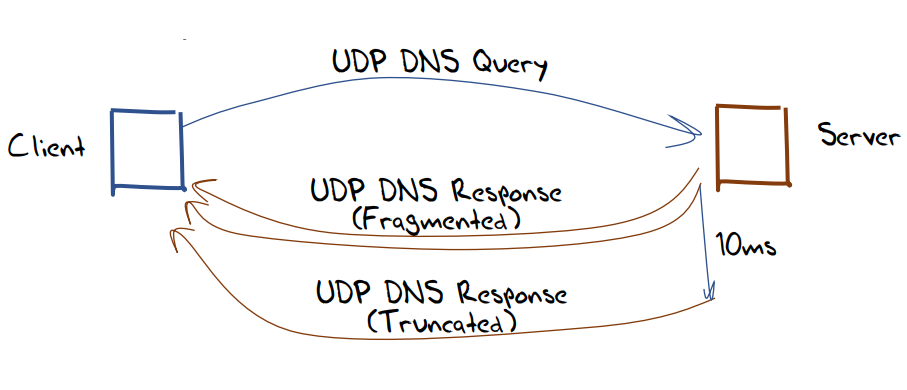
\includegraphics[width=\linewidth]{figures/ATR_a.png}
\caption{If fragment is not dropped} \label{fig:1a}
\end{subfigure}
\hspace*{\fill} % separation between the subfigures
\begin{subfigure}[b]{0.45\textwidth}
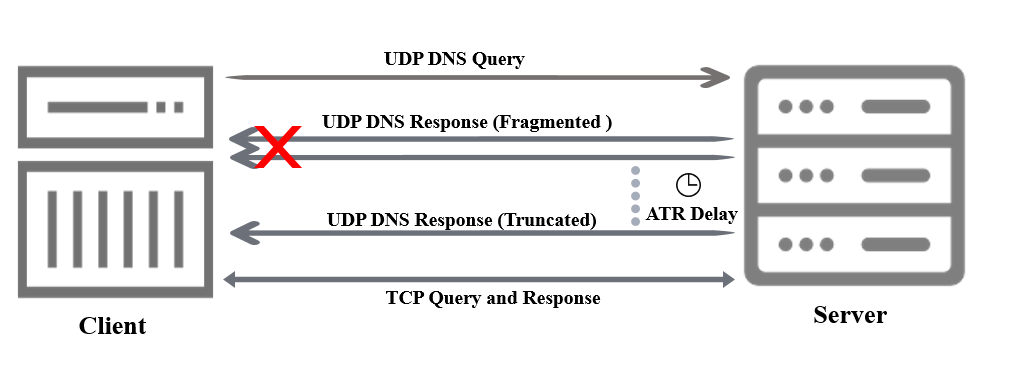
\includegraphics[width=\linewidth]{figures/ATR_b.png}
\caption{If fragment is dropped} \label{fig:1b}
\end{subfigure}
\caption{Operation of ATR} \label{fig:1}
\end{figure}


An approach to address this challenge is proposed in this section
called ATR (Additional Truncated Response). ATR mechanism is simple
that if a DNS server provides a response that entails sending
fragmented UDP packets, then the server should wait for a 10 ms
period and also back the original query as a truncated response.
If the client receives and reassembles the fragmented UDP response,
then the ensuing truncated response will be ignored by the client��s
DNS resolver as its outstanding query has already been answered.
If the fragmented UDP response is dropped by the network, then the
truncated response will be received (as it is far smaller), and
reception of this truncated response will trigger the client to
switch immediately to re-query using TCP without further delay.
This behavior is illustrated in Figure \ref{fig:1}.

\subsection{ATR Algorithm}

As show in the Figure \ref{fig:2} the ATR module can be implemented is right after truncation loop if the packet is not going to be fragmented.

\begin{figure}[tp]
\centering
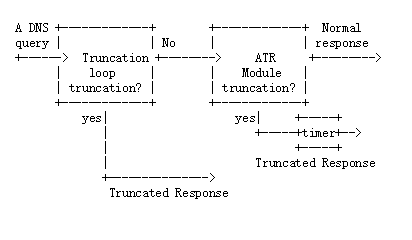
\includegraphics[width=\linewidth]{figures/ATR_Algorithm.png}
\caption{ATR module in DNS response process}\label{fig:2}
\end{figure}

The ATR responding process goes as follows:

\begin{itemize}
  \item When an authoritative server receives a query and enters the
      responding process, it first go through the normal truncation loop
      to see whether the size of response surpasses the EDNS0 payload
      size.  If yes, it ends up with responding a truncated packets.  If
      no, it enters the ATR module.
  \item In ATR module, similar like truncation loop, the size of response
      is compared with a value called ATR payload size.  If the response
      of a query is larger than ATR payload size, the server firstly
      sends the normal response and then coin a truncated response with
      the same ID of the query.
  \item The server can reply the coined truncated response in no time.
      But considering the possible impact of network reordering, it is
      suggested a timer to delay the second truncated response, for
      example 10~50 millisecond which can be configured by local
      operation.
\end{itemize}

   Note that the choice of ATR payload size and timer SHOULD be
   configured locally.  And the operational consideration and guidance
   is discussed following sections.

   There are three typical cases of ATR-unaware resolver behavior when a
   resolver send query to an ATR server in which the server will
   generate a large response with fragments:

   \begin{itemize}
  \item Case 1: a resolver (or sub-resolver) will receive both the large
   response and a very small truncated response in sequence.  It will
   happily accepts the first response and drop the second one because
   the transaction is over.
  \item Case 2: In case a fragment is dropped in the middle, the resolver
   will end up with only receiving the small truncated response.  It
   will retry using TCP in no time.
  \item Case 3: For those (probably 30\%*17\% of them) who can not speak TCP
      and sitting behind a firewall stubbornly dropping fragments.  ATR can
      not help!
\end{itemize}

   In the case authoritative server truncated all response surpass
   certain value , for example setting IPv6-edns-size to 1220 octets,
   ATR will helpful for resolver with TCP capacity, because the resolver
   still has a fair chance to receive the large response.

   \subsubsection{ATR timer}

   TBD

   \subsubsection{ATR payload size}

   Regarding the operational choice for ATR payload size, there are some
   good input from APNIC study [scoring-dns-root]on how to react to
   large DNS payload for authoritative server.  The difference in ATR is
   that ATR focuses on the second response after the ordinary response.

   For IPv4 DNS server, it is suggested the study that do not truncate
   and fragment IPv4 UDP response with a payload up to 1472 octets which
   is Ethernet MTU(1500) minus the sum of IPv4 header(20) and UDP
   header(8).  The reason is to avoid gratuitously fragmenting outbound
   packets and TCP fallback at the source.

   In the case of ATR, the first ordinary response is emitted without
   knowing it be to fragmented or not on the path.  If a large value is
   set up to 1472 octets, payload size between 512 octets and the large
   value size will probably get fragmented by aggressive firewalls which
   leads losing the benefit of ATR.  If ATR payload size set exactly 512
   octets, in most of case ATR response and the single unfragmented
   packets are under a race at the risk of RO.

   Given IPv4 fragmentation issue is not so serious compared to IPv6, it
   is suggested in this memo to set ATR payload size 1472 octets which
   means ATR only fit large DNS response larger than 1500 octets in
   IPv4.

   For IPv6 DNS server, similar to IPv4, the APNIC study is suggested
   that do not truncate IPv6 UDP packets with a payload up to 1,452
   octets which is Ethernet MTU(1500) minus the sum of IPv6 header(40)
   and UDP header(8). 1452 octets is chosen to avoid TCP fallback in the
   context that most TCP MSS in the root server is not set probably at
   that time.

   In the case of ATR considering the second truncated response, a
   smaller size: 1232 octets, which is IPv6 MTU for most network
   devices(1280) minus the sum of IPv6 header(40) and UDP header(8),
   should be chosen as ATR payload size to trigger necessary TCP
   fallback.  As a complementary requirement with ATR, the TCP MSS
   should be set 1220 octets to avoid Packet Too Big ICMP message as
   suggested in the APNIC study.

   In short, it is recommended that in IPv4 ATR payload size SHOULD be
   1472 octets, and in IPv6 the value SHOULD be 1232 octets.

   \subsubsection{Less aggressiveness of ATR}

   There is a concern ATR sends TC=1 response too aggressively
   especially in the beginning of adoption.  ATR can be implemented as
   an optional and configurable feature at the disposal of authoritative
   server operator.  One of the idea to mitigate this aggressiveness,
   ATR may respond TC=1 responses at a low possibility, such as 10\%.

   Another way is to reply ATR response selectively.  It is observed
   that RO and IPv6 fragmentation issues are path specific and
   persistent due to the Internet components and middle box.  So it is
   reasonable to keep a ATR "Whitelist" by counting the retries and
   recording the IP destination address of that large response causing
   many retires.  ATR only acts to those queries from the IP address in
   the white list.

   \subsubsection{Security Consideration}

   There may be concerns on DDoS attack problem due to the fact that the
   ATR introduces multiple responses from authoritative server.  The
   extra packet is pretty small.  In the worst case, it's 50% more
   packets and they are small

   DNS cookies \cite{RFC7873} and RRL on authoritative may be possible
   solutions


\section{ATR Evaluation}

In theory ATR provide a fix as a hybrid approach to the issue of
IPv6 fragmentation in the DNS. However, in
operational level, we need more quantitative analysis how ATR actually
works. In this section we are going to address two major operational
concerns. Firstly, as introduced in prior section, ATR relies on TCP as "plan B" .
But it is reported not every client DNS system supports using
TCP to emit queries. So it is possible that ATR will not help in
this case. But it is unknown what is the portion of user behind
TCP-broken resolvers. Another aspect of concern of ATR is Network
level packet re-ordering(RO) which may cause the shorter truncated
response packet to overtake the fragmented response, causing an
inflated TCP load, and the potential for TCP loss to be triggered.

\subsection{Measurement on ATR}

\begin{table*}[t]
   \caption{ASNs of IPv4 Resolvers that do not followup when given a large UDP Response �C Top 10}
   \centering
\begin{tabular}{@{}rrrlr@{}}
\toprule
\multicolumn{1}{c}{\textbf{ASN}} & \multicolumn{1}{c}{\textbf{Use}} & \multicolumn{1}{c}{\textbf{Exp}} & \multicolumn{1}{c}{\textbf{AS Name}} & \multicolumn{1}{l}{\textbf{CC}} \\ \midrule
AS9644 & 0.78\% & 447,019 & SK Telecom & KR \\
AS701 & 0.70\% & 400,798 & UUNET- MCI Communications Services & US \\
AS17853 & 0.62\% & 357,335 & LGTELECOM & KR \\
AS4766 & 0.59\% & 340,334 & Korea Telecom & KR \\
AS4134 & 0.47\% & 267,995 & CHINANET-BACKBONE & CN \\
AS31034 & 0.47\% & 267,478 & ARUBA-ASN & IT \\
AS3786 & 0.39\% & 225,296 & DACOM Corporation & KR \\
AS36692 & 0.38\% & 217,306 & OPENDNS - OpenDNS & US \\
AS3215 & 0.33\% & 189,810 & Orange & FR \\
AS812 & 0.30\% & 169,699 & ROGERS COMMUNICATIONS & CA \\ \bottomrule
\end{tabular}
\label{tab:ASN-IPv4}
\end{table*}

\begin{table*}[t]
   \caption{ASNs of IPv6 Resolvers that do not followup when given a large UDP Response �C Top 10}
   \centering
\begin{tabular}{@{}rrrlr@{}}
\toprule
\multicolumn{1}{c}{\textbf{ASN}} & \multicolumn{1}{c}{\textbf{Use}} & \multicolumn{1}{c}{\textbf{Exp}} & \multicolumn{1}{c}{\textbf{AS Name}} & \multicolumn{1}{l}{\textbf{CC}} \\ \midrule
AS15169 & 40.60\% & 10,006,596 & Google & US \\
AS5650 & 0.90\% & 221,493 & Frontier Communications & US \\
AS36692 & 0.84\% & 206,143 & OpenDNS & US \\
AS812 & 0.78\% & 193,073 & Rogers Communications Canada & CA \\
AS20057 & 0.46\% & 114,440 & AT\&T Mobility LLC & US \\
AS3352 & 0.38\% & 92,925 & TELEFONICA DE ESPANA & ES \\
AS852 & 0.35\% & 85,043 & TELUS Communications Inc. & CA \\
AS55644 & 0.32\% & 80,032 & Idea Cellular Limited & IN \\
AS3320 & 0.25\% & 61,938 & DTAG Internet service provider operations & DE \\
AS4761 & 0.24\% & 60,019 & INDOSAT-INP-AP INDOSAT Internet Network Provider & ID \\ \bottomrule
\end{tabular}
\label{tab:ASN-IPv6}
\end{table*}

Using the same measurement technique described in section 3,
we constructed 6 tests:

\begin{itemize}
  \item The first pair of tests used ATR over IPv4 and IPv6.
  In this case we constructed a fragmented UDP response by
  appending a NULL Resource Record (RR) into the response as
  an additional record, generating a response of 1,600 octets.
  We configured the server to deliberately ignore the offered
  UDP buffer size (if any) and generated this UDP fragmented
  response in all cases. The server then queued up a truncated
  response that was fired off 10ms after the original response.
  \item The second pair of tests used just the large packet
  response in both IPv4 and IPv6. In this case the server was
  configured to send a large fragmented UDP response in all
  cases, and never generated a truncated response.
  \item The third pair of tests was just the truncated UDP
  response in IPv4 and IPv6. Irrespective of the offered UDP
  buffer size the server echoed the query with an empty
  response part and the truncated flag set.
      operation.
\end{itemize}

This allowed us to measure the extent to which large
fragmented UDP responses fail on the paths between our
authoritative name servers and the resolvers that pose
queries to these servers. It also allows us to measure
the extent to which these resolvers are capable of using
TCP when given a truncated response. We can also measure
the extent to which ATR uses the trailing truncated response.

We performed these tests using the same online advertisement
distribution network to deliver the test script across the Internet.
Over 55 million end points were collected with 113,087 IPv4 visible
resolvers and 20,878 IPv6 visible resolvers. Similar with Table \ref{tab:geo_Fail},
Table \ref{tab:ASN-IPv4} and Table \ref{tab:ASN-IPv6} shows
the network location of most impacted resolvers. Table
\ref{tab:fail_resolver} shows the results from this experiment
looking at the behavior of each IP resolver.

Some 40\% of the IPv4 resolvers failed to receive the large
fragmented UDP response, which is a disturbingly high number.
Perhaps even more disturbing is the observed IPv6 failure rate,
which is an astounding 50\% of these visible resolvers when
a server is sending the resolver a fragmented UDP response.

The TCP failure numbers are not quite as large, but again
they are surprisingly high. Some 21\% of the IPv4 resolvers
were incapable of completing the resolution task if they
were forced to use TCP. The IPv6 number is more than double,
with 45\% of the IPv6 resolvers running into problems when
attempting to use TCP.

\begin{table}[]
   \caption{Failure Rate of Visible Resolvers}
   \centering
\begin{tabular}{@{}rrrl@{}}
\toprule
\multicolumn{1}{c}{\textbf{Protocol}} & \multicolumn{1}{c}{\textbf{Fail Large UDP}} & \multicolumn{1}{c}{\textbf{Fail TCP}} & \textbf{Fail ATR} \\ \midrule
IPv4 & 40\% & 21\% & \multicolumn{1}{r}{29\%} \\
IPv6 & 50\% & 45\% & \multicolumn{1}{r}{45\%} \\ \bottomrule
\end{tabular}
\label{tab:fail_resolver}
\end{table}

\begin{table}[]
\caption{Failure Rate of users}
\begin{tabular}{@{}rrrr@{}}
\toprule
\multicolumn{1}{c}{\textbf{Protocol}} & \multicolumn{1}{c}{\textbf{Fail Large UDP}} & \multicolumn{1}{c}{\textbf{Fail TCP}} & \multicolumn{1}{l}{\textbf{Fail ATR}} \\ \midrule
IPv4 & 13\% & 4\% & 4\% \\
IPv6 & 21\% & 8\% & 6\% \\ \bottomrule
\end{tabular}
\label{tab:fail_user}
\end{table}

The ATR approach was seen to assist resolvers, and in IPv4 the
ATR loss rate was 29\%, indicating that a little over 10\% of
resolvers that were incapable of receiving a fragmented UDP
response were able to switch over the TCP and complete the task.
The IPv6 ATR failure rate was 45\%, a 5\% improvement over the
underlying fragmented UDP loss rate.

When looking at the DNS, counting the behavior of resolvers
should not be used to infer the impact on users. In the DNS
the most heavily used 10,000 resolvers by IP address are used
by more than 90\% of users. If we want to understand the impact
of ATR on DNS resolution behaviors, as experienced by users,
then we need to look at this measurement from the user perspective.

For this user perspective measurement, we count a ��success��
if any resolver invoked by the user can complete the DNS
resolution process, and a ��failure�� otherwise. The user
perspective results are shown in Table \ref{tab:fail_user}.

These results indicate that in 9\% of IPv4 cases the use of ATR
by the server will improve the speed of resolution of a fragmented
UDP response by signaling to the client an immediate switch to
TCP to perform a re-query. The IPv6 behavior would improve the
resolution times in 15\% of cases.The residual ATR failure
rates appear to be those cases where the DNS resolver lies
behind a configuration that discards both DNS responses using
fragmented UDP and DNS responses using TCP.

It is shown that ATR certainly looks attractive if the objective is
to improve the speed of DNS resolution when passing large DNS responses.
And ATR is incrementally deployable in favor of decision made by each
server operator.  The remaining issue is risk of RO by the choice of
the delay timer which is discussed fully in next subsection.


% 2 page from APNIC's ATR measuring article

\subsection{Analysis on Network re-ordering impact}

%Atlas analysis

As introduced in Section 2 ATR timer is a way to avoid the impact of
network reordering(RO).  The value of the timer is critical, because
if the delay is too short, the ATR response may be received earlier
than the fragmented response (the first piece), the resolver will
fall back to TCP bearing the cost which should have been avoided.  If
the delay is too long, the client may timeout and retry which negates
the incremental benefit of ATR.  Generally speaking, the delay of the
timer should be "long enough, but not too long".

To the best knowledge of author, the nature of RO is characterized as
follows hopefully helping ATR users understand RO and how to operate
ATR appropriately in RO context.

\begin{itemize}
  \item RO is mainly caused by the parallelism in Internet components and
   links other than network anomaly [Bennett].  It was observed that
   RO is highly related to the traffic load of Internet components.
   So RO will long exists as long as the traffic load continue
   increase and the parallelism is used to enhance network
   throughput.
  \item The probability of RO varies largely depending on the different
   tests samples.  Some work shown RO probability below 2\% [Paxson]
   [Tinta] and another work was above 90\% [Bennett].  But it is
   agreed that RO is site-dependent and path-dependent.  It is
   observed in that when RO happens, it is mostly exhibited
   consistently in a small percentages of the paths.  It is also
   observed that higher rates smaller packets were more prone to RO
   because the sending inter-spacing time was small.
  \item It was reported that the inter-arrival time of RO varies from a
   few milliseconds to multiple tens of milliseconds [Tinta].  And
   the larger the packet the larger the inter-arrival time, since
   larger packets will take longer to be transmitted.
\end{itemize}

Reasonably we can infer that firstly RO should be taken into account
because it long exists due to middle Internet components which can
not be avoided by end-to-end way.  Secondly the mixture of larger and
small packets in ATR case will increase the inter-arrival time of RO
as well as the its probability.  The good news is that the RO is
highly site specific and path specific, and persistent which means

the ATR operator is able to identify a few sites and paths, setup a
tunable timer setting for them, or just put them into a blacklist
without replying ATR response.

Based on the above analysis it is hard to provide a perfect value of
ATR timer for all ATR users due to the diversity of networks.  It
seems OK to set the timer with a range from ten to hundreds ms, just
below the timeout setting of typical resolver.  Is suggested that a
decision should be made as operator-specific according to the
statistic of the RTT of their users.  Some measurement shown
[Brownlee][Liang] the mean of response time is below 50 ms for the
sites with lots of anycast instance like L-root, .com and .net name
servers.  For that sites, delay less than 50 ms is appropriate.

%1 page from data analysis

\section{Cost analysis}
%one or half page
TBD
\section{Conclusion and Future work}
TBD


\bibliographystyle{ACM-Reference-Format}
\bibliography{reference}

\end{document}